% Options for packages loaded elsewhere
\PassOptionsToPackage{unicode}{hyperref}
\PassOptionsToPackage{hyphens}{url}
%
\documentclass[
  ignorenonframetext,
]{beamer}
\usepackage{pgfpages}
\setbeamertemplate{caption}[numbered]
\setbeamertemplate{caption label separator}{: }
\setbeamercolor{caption name}{fg=normal text.fg}
\beamertemplatenavigationsymbolsempty
% Prevent slide breaks in the middle of a paragraph
\widowpenalties 1 10000
\raggedbottom
\setbeamertemplate{part page}{
  \centering
  \begin{beamercolorbox}[sep=16pt,center]{part title}
    \usebeamerfont{part title}\insertpart\par
  \end{beamercolorbox}
}
\setbeamertemplate{section page}{
  \centering
  \begin{beamercolorbox}[sep=12pt,center]{part title}
    \usebeamerfont{section title}\insertsection\par
  \end{beamercolorbox}
}
\setbeamertemplate{subsection page}{
  \centering
  \begin{beamercolorbox}[sep=8pt,center]{part title}
    \usebeamerfont{subsection title}\insertsubsection\par
  \end{beamercolorbox}
}
\AtBeginPart{
  \frame{\partpage}
}
\AtBeginSection{
  \ifbibliography
  \else
    \frame{\sectionpage}
  \fi
}
\AtBeginSubsection{
  \frame{\subsectionpage}
}

\usepackage{amsmath,amssymb}
\usepackage{iftex}
\ifPDFTeX
  \usepackage[T1]{fontenc}
  \usepackage[utf8]{inputenc}
  \usepackage{textcomp} % provide euro and other symbols
\else % if luatex or xetex
  \usepackage{unicode-math}
  \defaultfontfeatures{Scale=MatchLowercase}
  \defaultfontfeatures[\rmfamily]{Ligatures=TeX,Scale=1}
\fi
\usepackage{lmodern}
\ifPDFTeX\else  
    % xetex/luatex font selection
\fi
% Use upquote if available, for straight quotes in verbatim environments
\IfFileExists{upquote.sty}{\usepackage{upquote}}{}
\IfFileExists{microtype.sty}{% use microtype if available
  \usepackage[]{microtype}
  \UseMicrotypeSet[protrusion]{basicmath} % disable protrusion for tt fonts
}{}
\makeatletter
\@ifundefined{KOMAClassName}{% if non-KOMA class
  \IfFileExists{parskip.sty}{%
    \usepackage{parskip}
  }{% else
    \setlength{\parindent}{0pt}
    \setlength{\parskip}{6pt plus 2pt minus 1pt}}
}{% if KOMA class
  \KOMAoptions{parskip=half}}
\makeatother
\usepackage{xcolor}
\newif\ifbibliography
\setlength{\emergencystretch}{3em} % prevent overfull lines
\setcounter{secnumdepth}{-\maxdimen} % remove section numbering


\providecommand{\tightlist}{%
  \setlength{\itemsep}{0pt}\setlength{\parskip}{0pt}}\usepackage{longtable,booktabs,array}
\usepackage{calc} % for calculating minipage widths
\usepackage{caption}
% Make caption package work with longtable
\makeatletter
\def\fnum@table{\tablename~\thetable}
\makeatother
\usepackage{graphicx}
\makeatletter
\def\maxwidth{\ifdim\Gin@nat@width>\linewidth\linewidth\else\Gin@nat@width\fi}
\def\maxheight{\ifdim\Gin@nat@height>\textheight\textheight\else\Gin@nat@height\fi}
\makeatother
% Scale images if necessary, so that they will not overflow the page
% margins by default, and it is still possible to overwrite the defaults
% using explicit options in \includegraphics[width, height, ...]{}
\setkeys{Gin}{width=\maxwidth,height=\maxheight,keepaspectratio}
% Set default figure placement to htbp
\makeatletter
\def\fps@figure{htbp}
\makeatother
% definitions for citeproc citations
\NewDocumentCommand\citeproctext{}{}
\NewDocumentCommand\citeproc{mm}{%
  \begingroup\def\citeproctext{#2}\cite{#1}\endgroup}
\makeatletter
 % allow citations to break across lines
 \let\@cite@ofmt\@firstofone
 % avoid brackets around text for \cite:
 \def\@biblabel#1{}
 \def\@cite#1#2{{#1\if@tempswa , #2\fi}}
\makeatother
\newlength{\cslhangindent}
\setlength{\cslhangindent}{1.5em}
\newlength{\csllabelwidth}
\setlength{\csllabelwidth}{3em}
\newenvironment{CSLReferences}[2] % #1 hanging-indent, #2 entry-spacing
 {\begin{list}{}{%
  \setlength{\itemindent}{0pt}
  \setlength{\leftmargin}{0pt}
  \setlength{\parsep}{0pt}
  % turn on hanging indent if param 1 is 1
  \ifodd #1
   \setlength{\leftmargin}{\cslhangindent}
   \setlength{\itemindent}{-1\cslhangindent}
  \fi
  % set entry spacing
  \setlength{\itemsep}{#2\baselineskip}}}
 {\end{list}}
\usepackage{calc}
\newcommand{\CSLBlock}[1]{\hfill\break\parbox[t]{\linewidth}{\strut\ignorespaces#1\strut}}
\newcommand{\CSLLeftMargin}[1]{\parbox[t]{\csllabelwidth}{\strut#1\strut}}
\newcommand{\CSLRightInline}[1]{\parbox[t]{\linewidth - \csllabelwidth}{\strut#1\strut}}
\newcommand{\CSLIndent}[1]{\hspace{\cslhangindent}#1}

\usepackage{fontspec}
\usepackage{multirow}
\usepackage{multicol}
\usepackage{colortbl}
\usepackage{hhline}
\newlength\Oldarrayrulewidth
\newlength\Oldtabcolsep
\usepackage{longtable}
\usepackage{array}
\usepackage{hyperref}
\usepackage{float}
\usepackage{wrapfig}
\makeatletter
\@ifpackageloaded{tcolorbox}{}{\usepackage[skins,breakable]{tcolorbox}}
\@ifpackageloaded{fontawesome5}{}{\usepackage{fontawesome5}}
\definecolor{quarto-callout-color}{HTML}{909090}
\definecolor{quarto-callout-note-color}{HTML}{0758E5}
\definecolor{quarto-callout-important-color}{HTML}{CC1914}
\definecolor{quarto-callout-warning-color}{HTML}{EB9113}
\definecolor{quarto-callout-tip-color}{HTML}{00A047}
\definecolor{quarto-callout-caution-color}{HTML}{FC5300}
\definecolor{quarto-callout-color-frame}{HTML}{acacac}
\definecolor{quarto-callout-note-color-frame}{HTML}{4582ec}
\definecolor{quarto-callout-important-color-frame}{HTML}{d9534f}
\definecolor{quarto-callout-warning-color-frame}{HTML}{f0ad4e}
\definecolor{quarto-callout-tip-color-frame}{HTML}{02b875}
\definecolor{quarto-callout-caution-color-frame}{HTML}{fd7e14}
\makeatother
\makeatletter
\@ifpackageloaded{caption}{}{\usepackage{caption}}
\AtBeginDocument{%
\ifdefined\contentsname
  \renewcommand*\contentsname{Table of contents}
\else
  \newcommand\contentsname{Table of contents}
\fi
\ifdefined\listfigurename
  \renewcommand*\listfigurename{List of Figures}
\else
  \newcommand\listfigurename{List of Figures}
\fi
\ifdefined\listtablename
  \renewcommand*\listtablename{List of Tables}
\else
  \newcommand\listtablename{List of Tables}
\fi
\ifdefined\figurename
  \renewcommand*\figurename{Figure}
\else
  \newcommand\figurename{Figure}
\fi
\ifdefined\tablename
  \renewcommand*\tablename{Table}
\else
  \newcommand\tablename{Table}
\fi
}
\@ifpackageloaded{float}{}{\usepackage{float}}
\floatstyle{ruled}
\@ifundefined{c@chapter}{\newfloat{codelisting}{h}{lop}}{\newfloat{codelisting}{h}{lop}[chapter]}
\floatname{codelisting}{Listing}
\newcommand*\listoflistings{\listof{codelisting}{List of Listings}}
\makeatother
\makeatletter
\makeatother
\makeatletter
\@ifpackageloaded{caption}{}{\usepackage{caption}}
\@ifpackageloaded{subcaption}{}{\usepackage{subcaption}}
\makeatother

\ifLuaTeX
  \usepackage{selnolig}  % disable illegal ligatures
\fi
\usepackage{bookmark}

\IfFileExists{xurl.sty}{\usepackage{xurl}}{} % add URL line breaks if available
\urlstyle{same} % disable monospaced font for URLs
\hypersetup{
  pdftitle={Generalized Linear Models},
  hidelinks,
  pdfcreator={LaTeX via pandoc}}


\title{Generalized Linear Models}
\subtitle{For Over-Dispersed Data}
\author{}
\date{}

\begin{document}
\frame{\titlepage}


\begin{frame}{Basics of Generalized Linear Models (GLMs)}
\protect\hypertarget{basics-of-generalized-linear-models-glms}{}
\begin{itemize}
\tightlist
\item
  GLMs are a flexible generalization of ordinary linear regression that
  allows for response variables that have error distribution models
  other than a normal distribution.
\item
  \textbf{Components of GLMs}:

  \begin{itemize}
  \tightlist
  \item
    \textbf{Random Component}: Specifies the distribution of the
    response variable (e.g., Normal, Binomial, Poisson).
  \item
    \textbf{Systematic Component}: A linear predictor, a combination of
    explanatory variables (predictors).
  \item
    \textbf{Link Function}: Connects the mean of the response variable
    to the linear predictor (e.g., identity, log, logit).
  \end{itemize}
\end{itemize}
\end{frame}

\begin{frame}{Common link functions and GLMS}
\protect\hypertarget{common-link-functions-and-glms}{}
\begin{itemize}
\tightlist
\item
  \textbf{Identity Link}: Used for normally distributed data (linear
  regression).
\item
  \textbf{Logit Link}: Used for binary outcome data (logistic
  regression).
\item
  \textbf{Log Link}: Used for count data (Poisson regression).
\item
  \textbf{Reciprocal Link}: Used for increasing rate that levels off
  (Gamma regression).
\end{itemize}
\end{frame}

\begin{frame}{Over-Dispersed Data}
\protect\hypertarget{over-dispersed-data}{}
\begin{itemize}
\tightlist
\item
  Over-dispersion in general refers to having variance greater than that
  assumed for the theoretical data model.\\
\item
  Over-dispersion can also refer to having a variance that is greater
  than the mean

  \begin{itemize}
  \tightlist
  \item
    Similarly equa-dispersion would refer to having variance equal to
    the mean.
  \end{itemize}
\end{itemize}

\begin{tcolorbox}[enhanced jigsaw, colbacktitle=quarto-callout-note-color!10!white, breakable, arc=.35mm, leftrule=.75mm, opacitybacktitle=0.6, titlerule=0mm, colframe=quarto-callout-note-color-frame, toptitle=1mm, left=2mm, bottomrule=.15mm, toprule=.15mm, coltitle=black, bottomtitle=1mm, title={Poisson regression}, rightrule=.15mm, opacityback=0, colback=white]

Poisson regression is the most popular method for modeling count data.
The Poisson distribution brings with it the assumption of
equa-dispersion that is often unsatisfied.

\end{tcolorbox}
\end{frame}

\begin{frame}{Common applicataions}
\protect\hypertarget{common-applicataions}{}
\begin{columns}[T]
\begin{column}{0.5\textwidth}
\begin{itemize}
\tightlist
\item
  Count data in Biology
\item
  Epidemiology
\item
  Finance
\item
  Insurance claims
\item
  Environmental studies
\item
  etc.
\end{itemize}
\end{column}

\begin{column}{0.5\textwidth}
\begin{center}
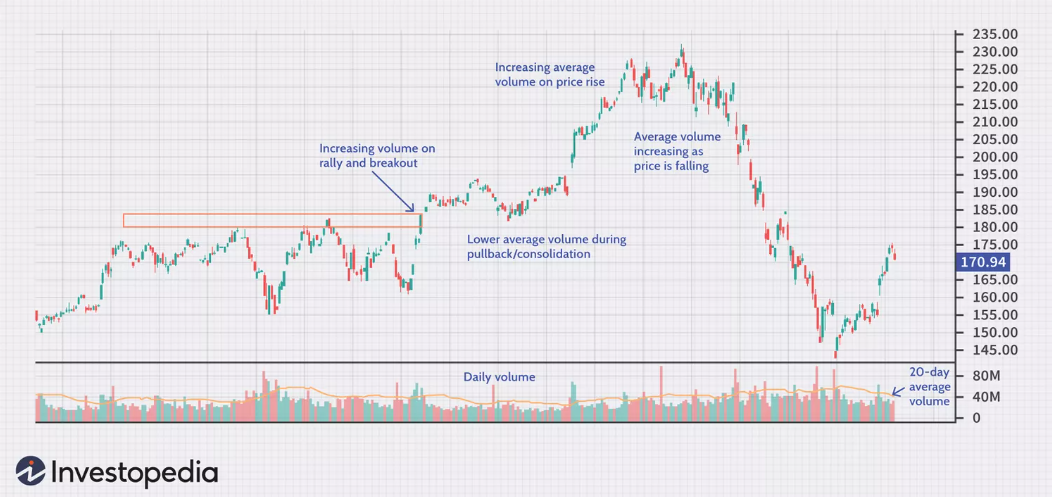
\includegraphics[width=0.8\textwidth,height=\textheight]{daily_stock_trades.png}
\end{center}

\begin{center}
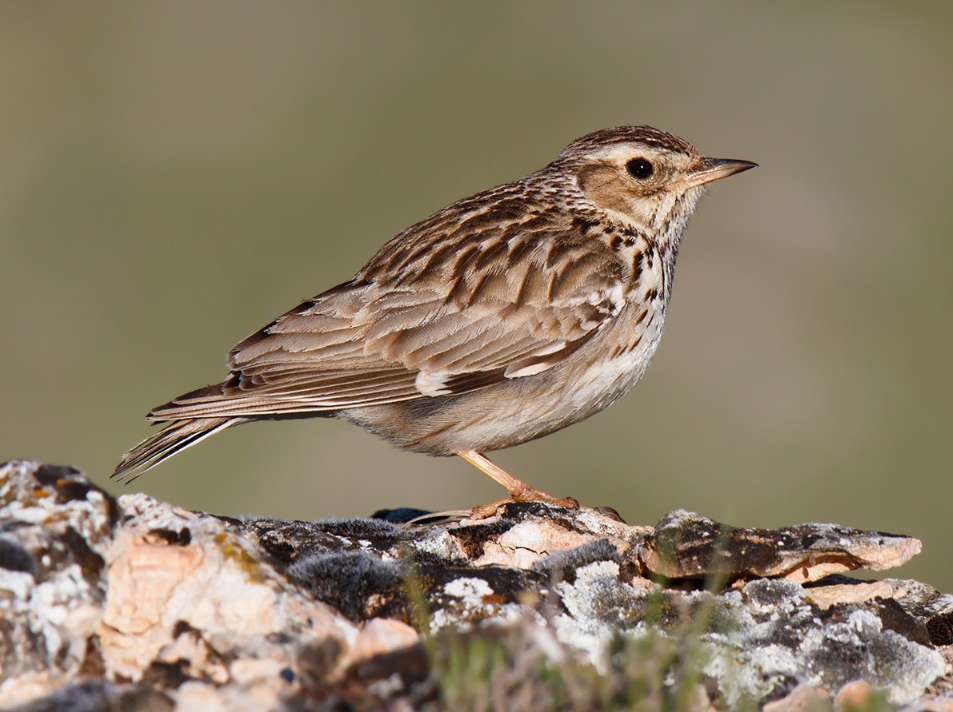
\includegraphics[width=0.5\textwidth,height=\textheight]{woodlark.png}
\end{center}
\end{column}
\end{columns}

Almost any real world count data is subject to the possibility of
over-dispersion.
\end{frame}

\begin{frame}{Causes}
\protect\hypertarget{causes}{}
\begin{columns}[T]
\begin{column}{0.5\textwidth}
\begin{itemize}
\tightlist
\item
  Increased variability of counts
\item
  Event clustering
\item
  Increased number of 0
\item
  Interaction effects
\item
  Measurement error
\item
  Environmental effects
\end{itemize}
\end{column}

\begin{column}{0.5\textwidth}
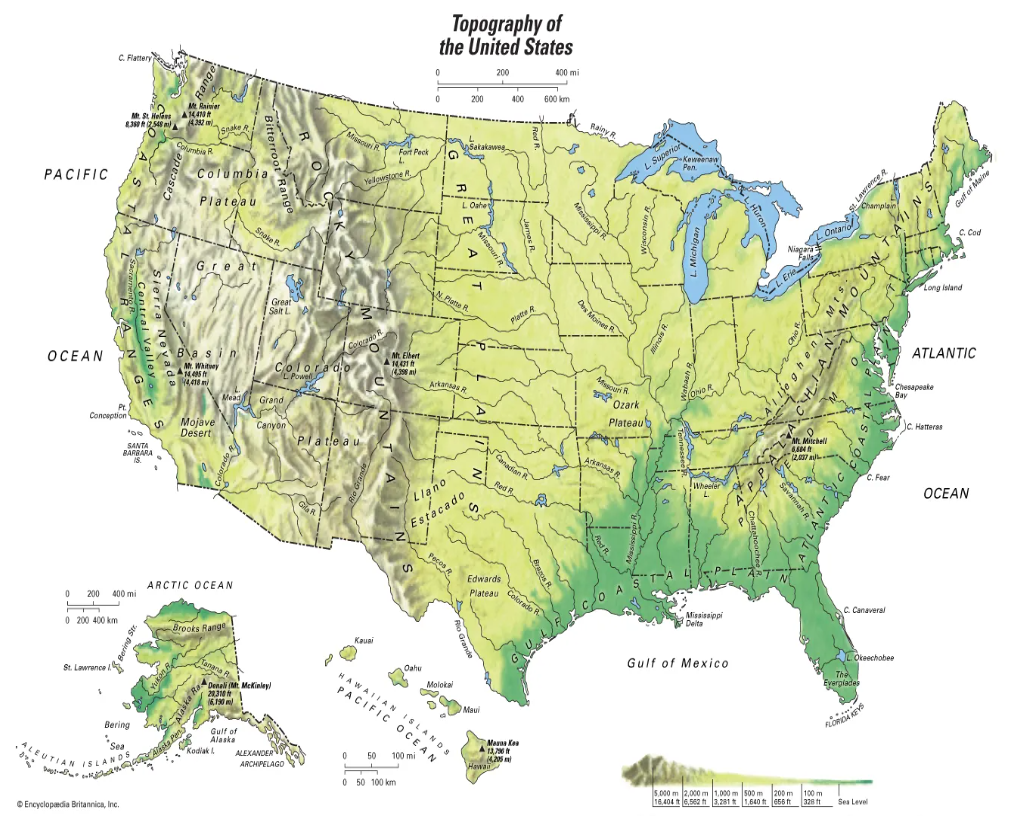
\includegraphics{topographic.png}
\end{column}
\end{columns}
\end{frame}

\begin{frame}{Candidate Distributions}
\protect\hypertarget{candidate-distributions}{}
\begin{enumerate}
\tightlist
\item
  Negative-Binomial
\item
  Generalized Poisson
\item
  Double Poisson
\item
  Conway-Maxwell-Poisson (CMP)
\end{enumerate}

\begin{itemize}
\tightlist
\item
  Zero inflated distributions

  \begin{itemize}
  \tightlist
  \item
    ZIP
  \item
    ZINB
  \item
    ZIDP/ZIGP
  \end{itemize}
\end{itemize}

\begin{columns}[T]
\begin{column}{0.5\textwidth}
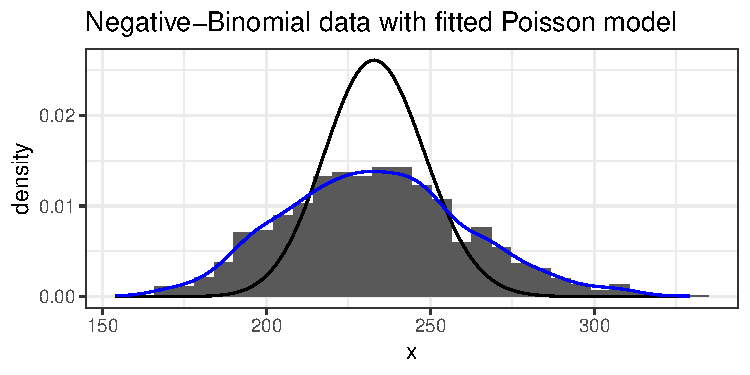
\includegraphics{cmp_pres_files/figure-beamer/unnamed-chunk-2-1.pdf}
\end{column}

\begin{column}{0.5\textwidth}
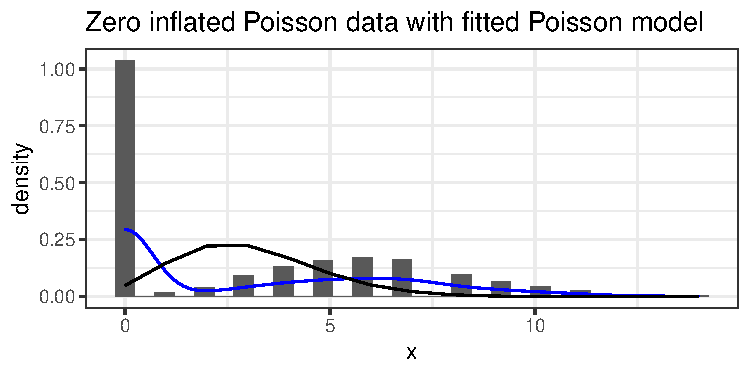
\includegraphics{cmp_pres_files/figure-beamer/unnamed-chunk-3-1.pdf}
\end{column}
\end{columns}
\end{frame}

\begin{frame}{Negative-Binomial}
\protect\hypertarget{negative-binomial}{}
\begin{itemize}
\tightlist
\item
  Parameters: mean: \(\mu\), dispersion: \(k\)\footnote<.->{The classic
    negative-binomial is parameterized as number of success and
    probability of success, \(r\) and \(p\).}
\item
  Variance: \(\mu + \mu^2/k\)

  \begin{itemize}
  \tightlist
  \item
    Function of mean and dispersion parameter
  \item
    Clearly captures over-dispersion.
  \end{itemize}
\end{itemize}
\end{frame}

\begin{frame}{Generalized Poisson}
\protect\hypertarget{generalized-poisson}{}
\begin{itemize}
\tightlist
\item
  Parameters: \(\lambda\), \(\theta\)
\item
  Mean: \(\lambda / (1- \theta) \quad\) Variance:
  \(\lambda / (1- \theta)^3\)
\item
  Model introduced by Consul 1989 as a way to modify the Poisson to
  handle over-dispersed and under-dispersed count data
\item
  Probability distribution function \[
  Pr(Y = y) = \frac{\lambda(\lambda + \theta y)^{y-1} e^{-(\lambda + \theta y)}}{y!}, \quad \lambda > 0,\space \theta \in \mathbb{R}
  \]
\end{itemize}

\begin{center}
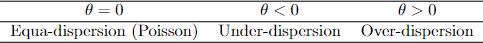
\includegraphics[width=0.5\textwidth,height=\textheight]{gp_table.png}
\end{center}
\end{frame}

\begin{frame}{Double Poisson}
\protect\hypertarget{double-poisson}{}
\begin{itemize}
\tightlist
\item
  Parameters: \(\mu\), \(\theta\)
\item
  Mean: \(\mu \quad\) Variance:\footnote<.->{Over-dispersed for
    \((\theta < 1)\), under-dispersed for \((\theta > 1)\),
    Poisson\((\theta = 1)\)} \(\mu / \theta\)
\item
  Extension of the double exponential family (Efron 1986) with
  approximate pmf \[
  Pr(Y = y) = (\theta^{1/2}e^{-\theta\mu}) \left(\frac{e^{y}y^y}{y!}\right) \left(\frac{e \mu}{y}\right)^{\theta y}
  \]
\item
  The exact double Poisson (DP) density includes a normalizing constant
  \(\sum_{y=0}^{\infty} Pr(Y = y) \approx 1 + \frac{1 - \theta}{12\mu\theta}(1 + \frac{1}{\mu\theta})\)
\end{itemize}
\end{frame}

\begin{frame}{Conway-Maxwell Poisson (CMP)}
\protect\hypertarget{conway-maxwell-poisson-cmp}{}
\begin{itemize}
\tightlist
\item
  Parameters:\footnote<.->{A mean parameterized CMP was introduced with
    better interpretation and computation (Huang 2017)} \(\lambda\),
  \(\nu\)
\item
  Mean: \(\mu \approx \lambda + 1/2\nu - 1/2 \quad\)
  Variance:\footnote<.->{Approximations only accurate under specific
    conditions \(\lambda > 10^\nu\) or \(\nu \le 1\) (Sellers et al.
    2012)} \(\sigma^2 \approx \lambda / \nu\)
\item
  Weighted Poison distribution with pmf: \[
  Pr(Y = y) = \frac{\lambda^y}{(y!)^\nu Z(\lambda, \nu)}, \quad Z(\lambda, \nu) = \sum_{y=0}^\infty \frac{\lambda^y}{(y!)^\nu}
  \]
\item
  Includes spacial cases (Sellers et al. 2012) of Poison when
  \(\nu = 1\), geometric when \(\nu \to 0\), and Bernoulli when
  \(\nu \to \infty\)
\end{itemize}
\end{frame}

\begin{frame}[fragile]{Zero Inflated Distributions}
\protect\hypertarget{zero-inflated-distributions}{}
\begin{itemize}
\tightlist
\item
  Zero inflated distributions are piece-wise distributions with
  components for 0s and non-0s
\item
  For example the zero inflated Poisson (ZIP) has pmf \[
  Pr(Y = y) = \cases{
  \pi + (1-\pi)e^{-\lambda} &\text{if } y = 0\\
  (1 - \pi)\frac{\lambda^y e^{-\lambda}}{y!} &\text{if } y = 1, 2, \ldots
  }
  \]
\item
  Zero inflated framework extends to other distributions to further
  capture over-dispersion and zero inflation
\item
  Models can be fit using the \texttt{zeroinfl()} function in the
  package \texttt{pscl}
\end{itemize}
\end{frame}

\begin{frame}{Model comparisons}
\protect\hypertarget{model-comparisons}{}
\begin{itemize}
\tightlist
\item
  2008 Bayesian paper compares the Generalized Poisson distribution,
  (Gschlößl and Czado 2008)
\end{itemize}

\global\setlength{\Oldarrayrulewidth}{\arrayrulewidth}

\global\setlength{\Oldtabcolsep}{\tabcolsep}

\setlength{\tabcolsep}{2pt}

\renewcommand*{\arraystretch}{1.5}



\providecommand{\ascline}[3]{\noalign{\global\arrayrulewidth #1}\arrayrulecolor[HTML]{#2}\cline{#3}}

\begin{longtable*}[c]{|p{0.75in}|p{0.75in}|p{0.75in}|p{0.75in}}



\ascline{1.5pt}{666666}{1-4}

\multicolumn{1}{>{\raggedright}m{\dimexpr 0.75in+0\tabcolsep}}{\textcolor[HTML]{000000}{\fontsize{11}{11}\selectfont{\global\setmainfont{DejaVu Sans}{Model}}}} & \multicolumn{1}{>{\raggedleft}m{\dimexpr 0.75in+0\tabcolsep}}{\textcolor[HTML]{000000}{\fontsize{11}{11}\selectfont{\global\setmainfont{DejaVu Sans}{Poisson}}}} & \multicolumn{1}{>{\raggedleft}m{\dimexpr 0.75in+0\tabcolsep}}{\textcolor[HTML]{000000}{\fontsize{11}{11}\selectfont{\global\setmainfont{DejaVu Sans}{NB}}}} & \multicolumn{1}{>{\raggedleft}m{\dimexpr 0.75in+0\tabcolsep}}{\textcolor[HTML]{000000}{\fontsize{11}{11}\selectfont{\global\setmainfont{DejaVu Sans}{GP}}}} \\

\ascline{1.5pt}{666666}{1-4}\endfirsthead 

\ascline{1.5pt}{666666}{1-4}

\multicolumn{1}{>{\raggedright}m{\dimexpr 0.75in+0\tabcolsep}}{\textcolor[HTML]{000000}{\fontsize{11}{11}\selectfont{\global\setmainfont{DejaVu Sans}{Model}}}} & \multicolumn{1}{>{\raggedleft}m{\dimexpr 0.75in+0\tabcolsep}}{\textcolor[HTML]{000000}{\fontsize{11}{11}\selectfont{\global\setmainfont{DejaVu Sans}{Poisson}}}} & \multicolumn{1}{>{\raggedleft}m{\dimexpr 0.75in+0\tabcolsep}}{\textcolor[HTML]{000000}{\fontsize{11}{11}\selectfont{\global\setmainfont{DejaVu Sans}{NB}}}} & \multicolumn{1}{>{\raggedleft}m{\dimexpr 0.75in+0\tabcolsep}}{\textcolor[HTML]{000000}{\fontsize{11}{11}\selectfont{\global\setmainfont{DejaVu Sans}{GP}}}} \\

\ascline{1.5pt}{666666}{1-4}\endhead



\multicolumn{1}{>{\raggedright}m{\dimexpr 0.75in+0\tabcolsep}}{\textcolor[HTML]{000000}{\fontsize{11}{11}\selectfont{\global\setmainfont{DejaVu Sans}{DIC}}}} & \multicolumn{1}{>{\raggedleft}m{\dimexpr 0.75in+0\tabcolsep}}{\textcolor[HTML]{000000}{\fontsize{11}{11}\selectfont{\global\setmainfont{DejaVu Sans}{1,291.8}}}} & \multicolumn{1}{>{\raggedleft}m{\dimexpr 0.75in+0\tabcolsep}}{\textcolor[HTML]{000000}{\fontsize{11}{11}\selectfont{\global\setmainfont{DejaVu Sans}{1,273.9}}}} & \multicolumn{1}{>{\raggedleft}m{\dimexpr 0.75in+0\tabcolsep}}{\textcolor[HTML]{000000}{\fontsize{11}{11}\selectfont{\global\setmainfont{DejaVu Sans}{1,265.6}}}} \\

\ascline{1.5pt}{666666}{1-4}



\end{longtable*}



\arrayrulecolor[HTML]{000000}

\global\setlength{\arrayrulewidth}{\Oldarrayrulewidth}

\global\setlength{\tabcolsep}{\Oldtabcolsep}

\renewcommand*{\arraystretch}{1}

\begin{itemize}
\tightlist
\item
  Car crash analysis using the DP and CMP model (Zou et al. 2013)
\end{itemize}

\global\setlength{\Oldarrayrulewidth}{\arrayrulewidth}

\global\setlength{\Oldtabcolsep}{\tabcolsep}

\setlength{\tabcolsep}{2pt}

\renewcommand*{\arraystretch}{1.5}



\providecommand{\ascline}[3]{\noalign{\global\arrayrulewidth #1}\arrayrulecolor[HTML]{#2}\cline{#3}}

\begin{longtable*}[c]{|p{0.75in}|p{0.75in}|p{0.75in}|p{0.75in}}



\ascline{1.5pt}{666666}{1-4}

\multicolumn{1}{>{\raggedright}m{\dimexpr 0.75in+0\tabcolsep}}{\textcolor[HTML]{000000}{\fontsize{11}{11}\selectfont{\global\setmainfont{DejaVu Sans}{Model}}}} & \multicolumn{1}{>{\raggedleft}m{\dimexpr 0.75in+0\tabcolsep}}{\textcolor[HTML]{000000}{\fontsize{11}{11}\selectfont{\global\setmainfont{DejaVu Sans}{DP}}}} & \multicolumn{1}{>{\raggedleft}m{\dimexpr 0.75in+0\tabcolsep}}{\textcolor[HTML]{000000}{\fontsize{11}{11}\selectfont{\global\setmainfont{DejaVu Sans}{NB}}}} & \multicolumn{1}{>{\raggedleft}m{\dimexpr 0.75in+0\tabcolsep}}{\textcolor[HTML]{000000}{\fontsize{11}{11}\selectfont{\global\setmainfont{DejaVu Sans}{CMP}}}} \\

\ascline{1.5pt}{666666}{1-4}\endfirsthead 

\ascline{1.5pt}{666666}{1-4}

\multicolumn{1}{>{\raggedright}m{\dimexpr 0.75in+0\tabcolsep}}{\textcolor[HTML]{000000}{\fontsize{11}{11}\selectfont{\global\setmainfont{DejaVu Sans}{Model}}}} & \multicolumn{1}{>{\raggedleft}m{\dimexpr 0.75in+0\tabcolsep}}{\textcolor[HTML]{000000}{\fontsize{11}{11}\selectfont{\global\setmainfont{DejaVu Sans}{DP}}}} & \multicolumn{1}{>{\raggedleft}m{\dimexpr 0.75in+0\tabcolsep}}{\textcolor[HTML]{000000}{\fontsize{11}{11}\selectfont{\global\setmainfont{DejaVu Sans}{NB}}}} & \multicolumn{1}{>{\raggedleft}m{\dimexpr 0.75in+0\tabcolsep}}{\textcolor[HTML]{000000}{\fontsize{11}{11}\selectfont{\global\setmainfont{DejaVu Sans}{CMP}}}} \\

\ascline{1.5pt}{666666}{1-4}\endhead



\multicolumn{1}{>{\raggedright}m{\dimexpr 0.75in+0\tabcolsep}}{\textcolor[HTML]{000000}{\fontsize{11}{11}\selectfont{\global\setmainfont{DejaVu Sans}{AIC}}}} & \multicolumn{1}{>{\raggedleft}m{\dimexpr 0.75in+0\tabcolsep}}{\textcolor[HTML]{000000}{\fontsize{11}{11}\selectfont{\global\setmainfont{DejaVu Sans}{3,268.20}}}} & \multicolumn{1}{>{\raggedleft}m{\dimexpr 0.75in+0\tabcolsep}}{\textcolor[HTML]{000000}{\fontsize{11}{11}\selectfont{\global\setmainfont{DejaVu Sans}{3,199.200}}}} & \multicolumn{1}{>{\raggedleft}m{\dimexpr 0.75in+0\tabcolsep}}{\textcolor[HTML]{000000}{\fontsize{11}{11}\selectfont{\global\setmainfont{DejaVu Sans}{}}}} \\





\multicolumn{1}{>{\raggedright}m{\dimexpr 0.75in+0\tabcolsep}}{\textcolor[HTML]{000000}{\fontsize{11}{11}\selectfont{\global\setmainfont{DejaVu Sans}{MSPE}}}} & \multicolumn{1}{>{\raggedleft}m{\dimexpr 0.75in+0\tabcolsep}}{\textcolor[HTML]{000000}{\fontsize{11}{11}\selectfont{\global\setmainfont{DejaVu Sans}{2.62}}}} & \multicolumn{1}{>{\raggedleft}m{\dimexpr 0.75in+0\tabcolsep}}{\textcolor[HTML]{000000}{\fontsize{11}{11}\selectfont{\global\setmainfont{DejaVu Sans}{2.727}}}} & \multicolumn{1}{>{\raggedleft}m{\dimexpr 0.75in+0\tabcolsep}}{\textcolor[HTML]{000000}{\fontsize{11}{11}\selectfont{\global\setmainfont{DejaVu Sans}{2.73}}}} \\

\ascline{1.5pt}{666666}{1-4}



\end{longtable*}



\arrayrulecolor[HTML]{000000}

\global\setlength{\arrayrulewidth}{\Oldarrayrulewidth}

\global\setlength{\tabcolsep}{\Oldtabcolsep}

\renewcommand*{\arraystretch}{1}

\begin{itemize}
\tightlist
\item
  Bayesian paper compared Poisson, Negative Binomial, and CMP for
  longitudinal counts using DIC to compare. (Alam et al. 2023)
\end{itemize}

\global\setlength{\Oldarrayrulewidth}{\arrayrulewidth}

\global\setlength{\Oldtabcolsep}{\tabcolsep}

\setlength{\tabcolsep}{2pt}

\renewcommand*{\arraystretch}{1.5}



\providecommand{\ascline}[3]{\noalign{\global\arrayrulewidth #1}\arrayrulecolor[HTML]{#2}\cline{#3}}

\begin{longtable*}[c]{|p{0.75in}|p{0.75in}|p{0.75in}|p{0.75in}}



\ascline{1.5pt}{666666}{1-4}

\multicolumn{1}{>{\raggedright}m{\dimexpr 0.75in+0\tabcolsep}}{\textcolor[HTML]{000000}{\fontsize{11}{11}\selectfont{\global\setmainfont{DejaVu Sans}{Model}}}} & \multicolumn{1}{>{\raggedleft}m{\dimexpr 0.75in+0\tabcolsep}}{\textcolor[HTML]{000000}{\fontsize{11}{11}\selectfont{\global\setmainfont{DejaVu Sans}{Poisson}}}} & \multicolumn{1}{>{\raggedleft}m{\dimexpr 0.75in+0\tabcolsep}}{\textcolor[HTML]{000000}{\fontsize{11}{11}\selectfont{\global\setmainfont{DejaVu Sans}{NB}}}} & \multicolumn{1}{>{\raggedleft}m{\dimexpr 0.75in+0\tabcolsep}}{\textcolor[HTML]{000000}{\fontsize{11}{11}\selectfont{\global\setmainfont{DejaVu Sans}{CMP}}}} \\

\ascline{1.5pt}{666666}{1-4}\endfirsthead 

\ascline{1.5pt}{666666}{1-4}

\multicolumn{1}{>{\raggedright}m{\dimexpr 0.75in+0\tabcolsep}}{\textcolor[HTML]{000000}{\fontsize{11}{11}\selectfont{\global\setmainfont{DejaVu Sans}{Model}}}} & \multicolumn{1}{>{\raggedleft}m{\dimexpr 0.75in+0\tabcolsep}}{\textcolor[HTML]{000000}{\fontsize{11}{11}\selectfont{\global\setmainfont{DejaVu Sans}{Poisson}}}} & \multicolumn{1}{>{\raggedleft}m{\dimexpr 0.75in+0\tabcolsep}}{\textcolor[HTML]{000000}{\fontsize{11}{11}\selectfont{\global\setmainfont{DejaVu Sans}{NB}}}} & \multicolumn{1}{>{\raggedleft}m{\dimexpr 0.75in+0\tabcolsep}}{\textcolor[HTML]{000000}{\fontsize{11}{11}\selectfont{\global\setmainfont{DejaVu Sans}{CMP}}}} \\

\ascline{1.5pt}{666666}{1-4}\endhead



\multicolumn{1}{>{\raggedright}m{\dimexpr 0.75in+0\tabcolsep}}{\textcolor[HTML]{000000}{\fontsize{11}{11}\selectfont{\global\setmainfont{DejaVu Sans}{DIC}}}} & \multicolumn{1}{>{\raggedleft}m{\dimexpr 0.75in+0\tabcolsep}}{\textcolor[HTML]{000000}{\fontsize{11}{11}\selectfont{\global\setmainfont{DejaVu Sans}{1,362.39}}}} & \multicolumn{1}{>{\raggedleft}m{\dimexpr 0.75in+0\tabcolsep}}{\textcolor[HTML]{000000}{\fontsize{11}{11}\selectfont{\global\setmainfont{DejaVu Sans}{1,350.67}}}} & \multicolumn{1}{>{\raggedleft}m{\dimexpr 0.75in+0\tabcolsep}}{\textcolor[HTML]{000000}{\fontsize{11}{11}\selectfont{\global\setmainfont{DejaVu Sans}{1,348.87}}}} \\

\ascline{1.5pt}{666666}{1-4}



\end{longtable*}



\arrayrulecolor[HTML]{000000}

\global\setlength{\arrayrulewidth}{\Oldarrayrulewidth}

\global\setlength{\tabcolsep}{\Oldtabcolsep}

\renewcommand*{\arraystretch}{1}
\end{frame}

\begin{frame}{Further Comparison}
\protect\hypertarget{further-comparison}{}
\begin{itemize}
\tightlist
\item
  Another Bayesian paper compared using AIC and shows the following
  results (Sellers and Shmueli 2010)
\end{itemize}

\global\setlength{\Oldarrayrulewidth}{\arrayrulewidth}

\global\setlength{\Oldtabcolsep}{\tabcolsep}

\setlength{\tabcolsep}{2pt}

\renewcommand*{\arraystretch}{1.5}



\providecommand{\ascline}[3]{\noalign{\global\arrayrulewidth #1}\arrayrulecolor[HTML]{#2}\cline{#3}}

\begin{longtable*}[c]{|p{0.75in}|p{0.75in}|p{0.75in}|p{0.75in}}



\ascline{1.5pt}{666666}{1-4}

\multicolumn{1}{>{\raggedright}m{\dimexpr 0.75in+0\tabcolsep}}{\textcolor[HTML]{000000}{\fontsize{11}{11}\selectfont{\global\setmainfont{DejaVu Sans}{Model}}}} & \multicolumn{1}{>{\raggedleft}m{\dimexpr 0.75in+0\tabcolsep}}{\textcolor[HTML]{000000}{\fontsize{11}{11}\selectfont{\global\setmainfont{DejaVu Sans}{CMP}}}} & \multicolumn{1}{>{\raggedleft}m{\dimexpr 0.75in+0\tabcolsep}}{\textcolor[HTML]{000000}{\fontsize{11}{11}\selectfont{\global\setmainfont{DejaVu Sans}{Poisson}}}} & \multicolumn{1}{>{\raggedleft}m{\dimexpr 0.75in+0\tabcolsep}}{\textcolor[HTML]{000000}{\fontsize{11}{11}\selectfont{\global\setmainfont{DejaVu Sans}{Neg-Bin}}}} \\

\ascline{1.5pt}{666666}{1-4}\endfirsthead 

\ascline{1.5pt}{666666}{1-4}

\multicolumn{1}{>{\raggedright}m{\dimexpr 0.75in+0\tabcolsep}}{\textcolor[HTML]{000000}{\fontsize{11}{11}\selectfont{\global\setmainfont{DejaVu Sans}{Model}}}} & \multicolumn{1}{>{\raggedleft}m{\dimexpr 0.75in+0\tabcolsep}}{\textcolor[HTML]{000000}{\fontsize{11}{11}\selectfont{\global\setmainfont{DejaVu Sans}{CMP}}}} & \multicolumn{1}{>{\raggedleft}m{\dimexpr 0.75in+0\tabcolsep}}{\textcolor[HTML]{000000}{\fontsize{11}{11}\selectfont{\global\setmainfont{DejaVu Sans}{Poisson}}}} & \multicolumn{1}{>{\raggedleft}m{\dimexpr 0.75in+0\tabcolsep}}{\textcolor[HTML]{000000}{\fontsize{11}{11}\selectfont{\global\setmainfont{DejaVu Sans}{Neg-Bin}}}} \\

\ascline{1.5pt}{666666}{1-4}\endhead



\multicolumn{1}{>{\raggedright}m{\dimexpr 0.75in+0\tabcolsep}}{\textcolor[HTML]{000000}{\fontsize{11}{11}\selectfont{\global\setmainfont{DejaVu Sans}{AIC}}}} & \multicolumn{1}{>{\raggedleft}m{\dimexpr 0.75in+0\tabcolsep}}{\textcolor[HTML]{000000}{\fontsize{11}{11}\selectfont{\global\setmainfont{DejaVu Sans}{5,073}}}} & \multicolumn{1}{>{\raggedleft}m{\dimexpr 0.75in+0\tabcolsep}}{\textcolor[HTML]{000000}{\fontsize{11}{11}\selectfont{\global\setmainfont{DejaVu Sans}{5,589}}}} & \multicolumn{1}{>{\raggedleft}m{\dimexpr 0.75in+0\tabcolsep}}{\textcolor[HTML]{000000}{\fontsize{11}{11}\selectfont{\global\setmainfont{DejaVu Sans}{5,077}}}} \\

\ascline{1.5pt}{666666}{1-4}



\end{longtable*}



\arrayrulecolor[HTML]{000000}

\global\setlength{\arrayrulewidth}{\Oldarrayrulewidth}

\global\setlength{\tabcolsep}{\Oldtabcolsep}

\renewcommand*{\arraystretch}{1}

\begin{itemize}
\tightlist
\item
  Mean parameterized CMP AIC and run time
\end{itemize}

\global\setlength{\Oldarrayrulewidth}{\arrayrulewidth}

\global\setlength{\Oldtabcolsep}{\tabcolsep}

\setlength{\tabcolsep}{2pt}

\renewcommand*{\arraystretch}{1.5}



\providecommand{\ascline}[3]{\noalign{\global\arrayrulewidth #1}\arrayrulecolor[HTML]{#2}\cline{#3}}

\begin{longtable*}[c]{|p{1.42in}|p{0.82in}|p{1.70in}|p{0.72in}}



\ascline{1.5pt}{666666}{1-4}

\multicolumn{1}{>{\raggedright}m{\dimexpr 1.42in+0\tabcolsep}}{\textcolor[HTML]{000000}{\fontsize{11}{11}\selectfont{\global\setmainfont{DejaVu Sans}{Model}}}} & \multicolumn{1}{>{\raggedleft}m{\dimexpr 0.82in+0\tabcolsep}}{\textcolor[HTML]{000000}{\fontsize{11}{11}\selectfont{\global\setmainfont{DejaVu Sans}{GP}}}} & \multicolumn{1}{>{\raggedleft}m{\dimexpr 1.7in+0\tabcolsep}}{\textcolor[HTML]{000000}{\fontsize{11}{11}\selectfont{\global\setmainfont{DejaVu Sans}{CMP(Mean-param)}}}} & \multicolumn{1}{>{\raggedleft}m{\dimexpr 0.72in+0\tabcolsep}}{\textcolor[HTML]{000000}{\fontsize{11}{11}\selectfont{\global\setmainfont{DejaVu Sans}{CMP}}}} \\

\ascline{1.5pt}{666666}{1-4}\endfirsthead 

\ascline{1.5pt}{666666}{1-4}

\multicolumn{1}{>{\raggedright}m{\dimexpr 1.42in+0\tabcolsep}}{\textcolor[HTML]{000000}{\fontsize{11}{11}\selectfont{\global\setmainfont{DejaVu Sans}{Model}}}} & \multicolumn{1}{>{\raggedleft}m{\dimexpr 0.82in+0\tabcolsep}}{\textcolor[HTML]{000000}{\fontsize{11}{11}\selectfont{\global\setmainfont{DejaVu Sans}{GP}}}} & \multicolumn{1}{>{\raggedleft}m{\dimexpr 1.7in+0\tabcolsep}}{\textcolor[HTML]{000000}{\fontsize{11}{11}\selectfont{\global\setmainfont{DejaVu Sans}{CMP(Mean-param)}}}} & \multicolumn{1}{>{\raggedleft}m{\dimexpr 0.72in+0\tabcolsep}}{\textcolor[HTML]{000000}{\fontsize{11}{11}\selectfont{\global\setmainfont{DejaVu Sans}{CMP}}}} \\

\ascline{1.5pt}{666666}{1-4}\endhead



\multicolumn{1}{>{\raggedright}m{\dimexpr 1.42in+0\tabcolsep}}{\textcolor[HTML]{000000}{\fontsize{11}{11}\selectfont{\global\setmainfont{DejaVu Sans}{AIC}}}} & \multicolumn{1}{>{\raggedleft}m{\dimexpr 0.82in+0\tabcolsep}}{\textcolor[HTML]{000000}{\fontsize{11}{11}\selectfont{\global\setmainfont{DejaVu Sans}{453.75}}}} & \multicolumn{1}{>{\raggedleft}m{\dimexpr 1.7in+0\tabcolsep}}{\textcolor[HTML]{000000}{\fontsize{11}{11}\selectfont{\global\setmainfont{DejaVu Sans}{440.82}}}} & \multicolumn{1}{>{\raggedleft}m{\dimexpr 0.72in+0\tabcolsep}}{\textcolor[HTML]{000000}{\fontsize{11}{11}\selectfont{\global\setmainfont{DejaVu Sans}{440.5}}}} \\





\multicolumn{1}{>{\raggedright}m{\dimexpr 1.42in+0\tabcolsep}}{\textcolor[HTML]{000000}{\fontsize{11}{11}\selectfont{\global\setmainfont{DejaVu Sans}{Run\ time\ (Sec)}}}} & \multicolumn{1}{>{\raggedleft}m{\dimexpr 0.82in+0\tabcolsep}}{\textcolor[HTML]{000000}{\fontsize{11}{11}\selectfont{\global\setmainfont{DejaVu Sans}{0.33}}}} & \multicolumn{1}{>{\raggedleft}m{\dimexpr 1.7in+0\tabcolsep}}{\textcolor[HTML]{000000}{\fontsize{11}{11}\selectfont{\global\setmainfont{DejaVu Sans}{8.50}}}} & \multicolumn{1}{>{\raggedleft}m{\dimexpr 0.72in+0\tabcolsep}}{\textcolor[HTML]{000000}{\fontsize{11}{11}\selectfont{\global\setmainfont{DejaVu Sans}{31.5}}}} \\

\ascline{1.5pt}{666666}{1-4}



\end{longtable*}



\arrayrulecolor[HTML]{000000}

\global\setlength{\arrayrulewidth}{\Oldarrayrulewidth}

\global\setlength{\tabcolsep}{\Oldtabcolsep}

\renewcommand*{\arraystretch}{1}

\begin{itemize}
\tightlist
\item
  Zero inflated Poisson regression model comparison for occupational
  injuries (Wang et al. 2003)
\end{itemize}

\global\setlength{\Oldarrayrulewidth}{\arrayrulewidth}

\global\setlength{\Oldtabcolsep}{\tabcolsep}

\setlength{\tabcolsep}{2pt}

\renewcommand*{\arraystretch}{1.5}



\providecommand{\ascline}[3]{\noalign{\global\arrayrulewidth #1}\arrayrulecolor[HTML]{#2}\cline{#3}}

\begin{longtable*}[c]{|p{1.39in}|p{0.97in}|p{0.97in}}



\ascline{1.5pt}{666666}{1-3}

\multicolumn{1}{>{\raggedright}m{\dimexpr 1.39in+0\tabcolsep}}{\textcolor[HTML]{000000}{\fontsize{11}{11}\selectfont{\global\setmainfont{DejaVu Sans}{Model}}}} & \multicolumn{1}{>{\raggedleft}m{\dimexpr 0.97in+0\tabcolsep}}{\textcolor[HTML]{000000}{\fontsize{11}{11}\selectfont{\global\setmainfont{DejaVu Sans}{Poisson}}}} & \multicolumn{1}{>{\raggedleft}m{\dimexpr 0.97in+0\tabcolsep}}{\textcolor[HTML]{000000}{\fontsize{11}{11}\selectfont{\global\setmainfont{DejaVu Sans}{ZIP}}}} \\

\ascline{1.5pt}{666666}{1-3}\endfirsthead 

\ascline{1.5pt}{666666}{1-3}

\multicolumn{1}{>{\raggedright}m{\dimexpr 1.39in+0\tabcolsep}}{\textcolor[HTML]{000000}{\fontsize{11}{11}\selectfont{\global\setmainfont{DejaVu Sans}{Model}}}} & \multicolumn{1}{>{\raggedleft}m{\dimexpr 0.97in+0\tabcolsep}}{\textcolor[HTML]{000000}{\fontsize{11}{11}\selectfont{\global\setmainfont{DejaVu Sans}{Poisson}}}} & \multicolumn{1}{>{\raggedleft}m{\dimexpr 0.97in+0\tabcolsep}}{\textcolor[HTML]{000000}{\fontsize{11}{11}\selectfont{\global\setmainfont{DejaVu Sans}{ZIP}}}} \\

\ascline{1.5pt}{666666}{1-3}\endhead



\multicolumn{1}{>{\raggedright}m{\dimexpr 1.39in+0\tabcolsep}}{\textcolor[HTML]{000000}{\fontsize{11}{11}\selectfont{\global\setmainfont{DejaVu Sans}{Log-Likelihood}}}} & \multicolumn{1}{>{\raggedleft}m{\dimexpr 0.97in+0\tabcolsep}}{\textcolor[HTML]{000000}{\fontsize{11}{11}\selectfont{\global\setmainfont{DejaVu Sans}{-409.678}}}} & \multicolumn{1}{>{\raggedleft}m{\dimexpr 0.97in+0\tabcolsep}}{\textcolor[HTML]{000000}{\fontsize{11}{11}\selectfont{\global\setmainfont{DejaVu Sans}{-397.704}}}} \\

\ascline{1.5pt}{666666}{1-3}



\end{longtable*}



\arrayrulecolor[HTML]{000000}

\global\setlength{\arrayrulewidth}{\Oldarrayrulewidth}

\global\setlength{\tabcolsep}{\Oldtabcolsep}

\renewcommand*{\arraystretch}{1}
\end{frame}

\begin{frame}[fragile]{Results}
\protect\hypertarget{results}{}
\begin{itemize}
\tightlist
\item
  It has been found and shown that modeling over-dispersed data with
  improper distributions leads to biased results.
\item
  To prevent biased results from over dispersed data, using models such
  as the CMP, GP, or DP model can prove beneficial
\item
  Zero inflated models have better fit when there are increased number
  of zeros observed and can easily be implemented
\item
  Some of these models are easy to implement such as the CMP and
  CMP(mean-parameterized) in packages \texttt{COMPoissonReg} and
  \texttt{mpcmp}
\end{itemize}
\end{frame}

\begin{frame}{References}
\protect\hypertarget{references}{}
\hypertarget{refs}{}
\begin{CSLReferences}{1}{0}
\leavevmode\vadjust pre{\hypertarget{ref-alam_bayesian_2023}{}}%
Alam, M., Gwon, Y., and Meza, J. (2023), {``Bayesian
conway-maxwell-poisson ({CMP}) regression for longitudinal count
data,''} \emph{Communications for Statistical Applications and Methods},
30, 291--309. \url{https://doi.org/10.29220/CSAM.2023.30.3.291}.

\leavevmode\vadjust pre{\hypertarget{ref-efron_double_1986}{}}%
Efron, B. (1986), {``Double exponential families and their use in
generalized linear regression,''} \emph{Journal of the American
Statistical Association}, 81, 709--721.
\url{https://doi.org/10.2307/2289002}.

\leavevmode\vadjust pre{\hypertarget{ref-gschlosl_modelling_2008}{}}%
Gschlößl, S., and Czado, C. (2008), {``Modelling count data with
overdispersion and spatial effects,''} \emph{Statistical Papers}, 49,
531--552. \url{https://doi.org/10.1007/s00362-006-0031-6}.

\leavevmode\vadjust pre{\hypertarget{ref-huang_mean-parametrized_2017}{}}%
Huang, A. (2017), {``Mean-parametrized {Conway}--{Maxwell}--{Poisson}
regression models for dispersed counts,''} \emph{Statistical Modelling},
17, 359--380. \url{https://doi.org/10.1177/1471082X17697749}.

\leavevmode\vadjust pre{\hypertarget{ref-sellers_com-poisson_2012}{}}%
Sellers, K. F., Borle, S., and Shmueli, G. (2012), {``The {COM}-poisson
model for count data: A survey of methods and applications,''}
\emph{Applied Stochastic Models in Business and Industry}, 28, 104--116.
\url{https://doi.org/10.1002/asmb.918}.

\leavevmode\vadjust pre{\hypertarget{ref-sellers_flexible_2010}{}}%
Sellers, K. F., and Shmueli, G. (2010),
{``\href{https://www.jstor.org/stable/29765537}{A flexible regression
model for count data},''} \emph{The Annals of Applied Statistics}, 4,
943--961.

\leavevmode\vadjust pre{\hypertarget{ref-wang_bivariate_2003}{}}%
Wang, K., Lee, A. H., Yau, K. K. W., and Carrivick, P. J. W. (2003),
{``A bivariate zero-inflated {Poisson} regression model to analyze
occupational injuries,''} \emph{Accident Analysis \& Prevention}, 35,
625--629. \url{https://doi.org/10.1016/S0001-4575(02)00036-2}.

\leavevmode\vadjust pre{\hypertarget{ref-zou_evaluating_2013}{}}%
Zou, Y., Geedipally, S. R., and Lord, D. (2013), {``Evaluating the
double poisson generalized linear model,''} \emph{Accident Analysis \&
Prevention}, 59, 497--505.
\url{https://doi.org/10.1016/j.aap.2013.07.017}.

\end{CSLReferences}
\end{frame}




\end{document}
